\documentclass[twocolumn]{article}

\usepackage[margin=1in]{geometry}
\usepackage{csquotes}
\usepackage{enumitem}

\usepackage{graphicx}

\title{Peer-to-Peer Wikipedia}
\author{Rain Gu and Nick Bradley}
\date{December 13, 2016}

\begin{document}
\maketitle

\begin{abstract}
We were motivated to create a peer-to-peer version of Wikipedia by our desire to remove proprietary interests in the online encyclopedia. Our prototype implements the Treedoc CRDT and an enhanced version of Chord with finger tables, replication and caching. These features allow our client application to support disconnected editing of articles without fear of losing local changes. Its design is scalable and robust to failures while maintaining article consistency and availability.
\end{abstract}

\section{Introduction}
Wikipedia is a free online collaborative encyclopedia funded and hosted by the non-profit Wikimedia foundation. In its current incarnation, Wikipedia is run in a typical client-server configuration giving Wikimedia full control of the content and infrastructure. To fund the administration costs, Wikimedia relies on public donations making it possible that Wikipedia could become permanently unavailable. By moving to a peer-to-peer version, we remove proprietary interests in the system and eliminate costs associated with administrating infrastructure. Both approaches require direct support from users: in the case of Wikipedia it is a monetary donation; in our peer-to-peer system, it is storage and network resources. It is an interesting question whether users prefer the former or later but we do not attempt to answer it.

The primary goal of a wiki, which promotes cooperative editing of articles of text, is to maintain the consistency of the article while making it available for editing to as many users as possible. Once the number of users increases, copies of articles may need to be hosted on multiple servers to ensure availability. Here, we briefly compare the client-server approach of Wikipedia to the peer-to-peer approach of our system.

Support for collaborative editing of articles hosted by Wikipedia could be provided in several different ways. They could use a commutative replicated data type (CRDT), as in our prototype, or they could serialize operations through a master server using a consensus protocol like Paxos \cite{paxos} or Raft \cite{raft}. Consensus protocols do not scale well, so they are most appropriate when used with a small number of servers.

To make its service more responsive, Wikipedia could either add more servers (scale out) or increase the resources available to its current servers (scale up). In our peer-to-peer version, we chose a protocol that is efficient in the number of messages it sends to ensure that the physical network can support many peers. However, we cannot directly increase the number of hosts (although peers must be willing to host articles if they want to view articles).

In this report, we detail our prototype peer-to-peer version of Wikipedia. It implements both an enhanced version of Chord \cite{c1} and the unoptimized version of Treedoc \cite{t1,t2}. Chord provides efficient article lookup by organizing the peers in the network. It handles peers joining the network as well as peer failure and churn. We base our articles on Treedoc, which guarantees that different versions of an article converge without concurrency control. Together, these provide a scalable system which supports highly available, (eventually) consistent articles.

The remainder of this report proceeds as follows. Section 2 provides background on the Chord protocol and the Treedoc CRDT. Section 3 details the challenges of running a collaborative wiki on a peer-to-peer network and limits the scope of the problem. Section 4 discusses our prototype system. Section 5 evaluates the prototype. Section 6 summarizes our conclusions and lists possible areas of future work.

\section{Background}
In this section, we review Chord \cite{c1} and Treedoc \cite{t1}. These are the fundamental components of our prototype.

\subsection{Chord}
Chord refers to both a protocol and an algorithm for managing a distributed hash table (DHT). All entities (peers and articles) are assigned an $m$-bit identifier\footnote{For $m$-bit identifiers, Chord supports $2^m-1$ entities.}, or \textit{key}, which is obtained using a consistent hashing function such as SHA-1. The key represents the entity's position in the Chord ring and allows us to determine on which peer each article should be stored. Peers are identified by hashing their IP addresses while articles are identified by hashing their titles. Each peer in the system maintains the IP address of its \textit{predecessor peer} (the peer immediately preceding it in the ring), its \textit{successor peer} (the peer immediately following it in the ring), and a portion of the key-value pairs in the DHT. The key-value pairs that are stored on a specific peer are those whose keys fall between its predecessor's key and its own key.

\subsubsection{Lookups}
When a peer wishes to retrieve a value from the DHT, it must do so by searching the network. Because of the Chord structure, lookups can be run in logarithmic time in the number of peers, $N$. When a peer initiates a lookup, it first checks to see if it or its successor is responsible for the lookup key. If not, it forwards the request to its successor which repeats the same process. This procedure repeats until the host peer is found, at which point its address is returned to the initiator. To reduce the search time, each node maintains a finger table consisting of $m$ IP addresses which act as a routing cache. Specifically, the $i$th entry in the finger table on peer with ID $n$ contains the ID of the first peer $f$ that succeeds $n$ by at least $2^{i-1}$, which is the successor of $n+2^{i-1}$. By maintaining the finger table, the lookup will \enquote{skip} to the closest peer in the table where it proceeds as before. This optimization reduces the total lookup time from $O(N)$ to $O(log⁡{N})$ with high probability.

\subsubsection{Joins and Exits}
A peer, $J$, wishing to join the network needs to know the IP address of another peer already in the network. This peer determines $J$'s position in the network and the IP address of its successor peer, $S$. Upon joining, $J$ will notify $S$ that it should be its new predecessor. Eventually, $S$'s predecessor will stabilize\footnote{Each peer will periodically run a \texttt{stabilize} procedure that will check if its successor's predecessor is still itself. If not, it will notify the new predecessor.}. Key-value pairs on $S$ that lie between $J$ and its predecessor must be transferred to $J$. Once this completes, $J$ is fully integrated into the network.

A peer can voluntarily leave the network by sending its key-value pairs to its successor and then notifying its predecessor and successor of its departure. Upon receiving the notifications, the peers will initiate their \texttt{stabilize} procedures.

\subsubsection{Failures}
Peer failures are detected automatically during the \texttt{stabilize} procedure. When a peer's successor does not respond to \texttt{stabilize} requests, it is considered failed. To allow for recovery in this situation, each peer maintains not just one successor, but a list of $r$ successors, where $r$ is a measure of fault tolerance. Then, when a peer detects that a successor has failed, it will notify the next successor in the list, thus repairing the network structure. Unfortunately, the key-value pairs stored on the failed node are lost. We address this issue in the next subsection.

\subsubsection{Replication}
In the vanilla version of Chord, each key-value pair is stored only on a single peer. If that peer is unavailable, its key-value pairs are not available to any other peers and, in the case of failure, the key-value pairs are permanently lost. Replication of the key-value pairs is thus necessary to avoid this situation. However, it adds complexity to the design and implementation as we now need to consider the number, location, and consistency of the replicas as well as the cost of maintaining the replicas.

There were several ways we could have chosen to implement replication. One way would be to replicate the key-value pairs to random peers in the system and, upon failure of the host peer, find the replica and put it on a new host peer (a peer in the successor list of the failed peer). This approach would require some mechanism for maintaining a sufficient number of replicas.

Instead, we decided to support replication by taking advantage of the peer's successor list: each successor stores replicas of all key-value pairs stored on the peer. This is a good method because it does not require maintaining any additional state about the system and it is controlled by the same parameter $r$ as the successor list. This means that replicas are as fault-tolerant as the underlying Chord system.

Replication of a peer's key-value pairs occurs during maintenance of its successor list. The peer will push the key-value pairs to all of the successors on the list. In our prototype, we maintain consistency of the replicas using a CRDT which requires no consensus among peers.

Now if a peer fails, its predecessor will notify the next available successor in its successor list as usual. This successor will have all of the key-value pairs that were originally owned by the failed peer; hence, no pair will be lost. If a peer joins the system, it will take over ownership of some replicated key-value pairs, as explained in section 2.1.2. It is still possible that key-value pairs may be lost if multiple successors fail before the \texttt{stabilize} procedure runs (e.g. during a regional network partition), but this can be mitigated by selecting larger values of $r$.

\subsection{Treedoc}
Treedoc is a CRDT that was designed to support cooperative text editing. It allows users located at different sites to modify a shared article by operating on a local copy and then sending the changes to other sites to be replayed. Since Treedoc is designed such that concurrent inserts commute with one another, copies of the article converge automatically without the need for complex concurrency control. Treedoc is presented to the user as a linear sequence of paragraphs.

\begin{figure}[tbh!]
  \centering
  \includegraphics[width=0.4\textwidth]{report/images/treedoc1}
  \caption{A Treedoc with inserts from multiple users dS, dC1 and dC3.\label{fig:treedoc_basic}}
\end{figure}

\subsubsection{Identifiers}
To provide commutative operations, Treedoc requires that every paragraph have an identifier and that the identifiers are unique, totally ordered, and stable. Further, the identifiers must come from a dense identifier space such that it is always possible to generate a new identifier between any two existing identifiers.

Treedoc uses an extended binary tree to provide a dense identifier space: paragraphs are stored as nodes in the tree and the path to each paragraph acts as its identifier. In addition, nodes include the identity of the user who made the insert. Paths, represented as bit strings where 0 represents a left branch and 1 represents a right branch, are unique and stable. They are ordered by walking the tree in infix order. A simple Treedoc is shown in figure \ref{fig:treedoc_basic}. The circled letters represent the paragraphs and the letters prefixed by \enquote{d} represent the identity of the user who made the insert. For example, the leftmost node has text \enquote{A}, was inserted by \enquote{dC1} and has ID [0(0:dC1)]. The article would be displayed as ABCDEF. Note that a more space-efficient implementation could be achieved by separating storage from identification (e.g. by storing the paragraphs as an array of (paragraph, path) pairs). In that case, the tree version would only need to exist to generate a new identifier for insertions.

A standard binary tree is not sufficient to represent concurrent inserts since different users may insert different paragraphs in the same position. To handle this case, the tree structure is extended by allowing each node to contain a list of \enquote{mini-nodes} as shown in figure \ref{fig:treedoc_full}. In case of concurrent inserts along the same path, the paragraphs are inserted as a mini-nodes. However, this violates the total ordering of identifiers requirement since the position in the list may be determined by the order of execution. Therefore, we order the mini-nodes by the user's identity.

The algorithm to generate a new path for insertion is simple. At a high level: assume a new node is to be inserted between $P$ and $F$, where $P$ comes before $F$ in infix order. If $P$ is an ancestor of $F$ in the tree then the new node should be inserted to the left of $F$. Otherwise, it should be inserted to the right of $P$. We refer the reader to \cite{t2} for details.

\begin{figure}[tbh!]
  \centering
  \includegraphics[width=0.4\textwidth]{report/images/treedoc2}
  \caption{A Treedoc with concurrently inserted paragraphs W and Y. \label{fig:treedoc_full}}
\end{figure}

\subsubsection{Operations}
The Treedoc structure is modified by the two edit operations:
\begin{itemize}
  \item \texttt{Insert(path, text)}: inserts the text into the tree at the specified path.
  \item \texttt{Delete(path)}: removes the paragraph at the specified path. The paragraph is not actually removed from the tree as other sites may reference it in a concurrent replay. Instead, a tombstone flag, which controls visibility, is set to prevent the paragraph from being displayed.
\end{itemize}

Commutativity of the operations is guaranteed as follows. For any two operations that refer to independent identifiers, the operations commute since their effect on the tree is independent of execution order. By the identifier uniqueness requirement, new identifiers will be independent, which implies that two concurrent insert operations commute. In cases where concurrent operations act on the same identifier, we must have that an insert happens before a delete, so they can never be concurrent. Similarly, a delete can never precede an insert for the same identifier, so they can never be concurrent. Finally, the delete operation is idempotent so its effect will be the same regardless of the execution order. This shows that the operations are commutative. Thus, articles at remotes sites will converge if the operations are replayed in the same order as the modifying site.


\section{Prototype Design}
Deploying a service in a peer-to-peer environment presents many challenges because of the scale of the system and the typically unreliable nature of peers. For our prototype, we focus on availability, scalability, and the consistency of articles.

In our system, ``availability'' means that once an article has been put on a host peer, any client peer can access it. This means that the article must be replicated on some other peers in the system so that the article will be accessible in the event that the primary host peer is unavailable (i.e., disconnected or not running the Chord service). The version of Chord presented in \cite{c1} was designed to scale to the level needed to support internet applications. Our enhanced version scales while supporting the required level of replication.

We introduce a caching mechanism to improve the availability and scalability of the original Chord protocol. When a peer modifies an article, in addition to sending the changes to the host peer, the cache of every peer on the lookup path is also updated. Since the cache update uses the existing lookup calls, it does not impact scalability. When a peer wishes to retrieve an article, the lookup procedure will return a cached version unless the peer explicitly requests a non-cached version. Cached articles are deleted after a set time to ensure that they do not diverge too much from each other. Our caching mechanism increases availability since an article will be accessible on more peers. It adds scalability by reducing the number of lookup messages required to retrieve an article while keeping the same number of lookup calls required to update the remote article.

Article consistency is achieved by using Treedoc CRDT, which ensures that all versions of an article converge. It does not require concurrency control. This feature further increases both the availability and the scalability of the system since modifications do not need to be serialized, which would add delay to the system. The automatic convergence of Treedoc makes our caching system trivial to implement. It should be noted that we only guarantee eventual consistency: once no more changes are made, all copies of the article will show the same content.

\subsection{Design Considerations}
We assume that peers:
\begin{itemize}
  \item Are non-Byzantine since malicious peers could break the Chord protocol.
  \item Fail at a rate slow enough that the Chord structure can be repaired between failures.
  \item Have a unique address that is fixed once they join the network. Addresses are used as user identities when tracking changes to articles and therefore must not change.
  \item Upon joining the system, know the IP address of at least one active peer in the network. One way to ensure this would be to provide an external service that would receive heartbeats from active peers and publish their IP address. A peer wishing to join would simply query this service. Since it is expected that peers will disconnect frequently, they should cache their predecessor and successor's IP addresses and only query the service if none of the cached peers are available.
\end{itemize}

Our prototype does not support deleting or renaming articles, nor does it support substring- or content-based lookups. Though we ran out of time to implement article deletion, this would likely be straightforward since there is only one host peer: attempts to modify a deleted article would fail and cached versions would not be updated\footnote{All replay logs would need to indicate whether they expect the article to exist so that deletions could be detected.}. The cache expiration policy ensures that eventually all copies of the article are removed from the system. As a workaround, users may simply delete all content within the article. Renaming articles is challenging, as the article title is used as the lookup key. One potential solution would be to include an independent title field in the article structure. Unfortunately, this would hamper the simple elegance of Treedoc by requiring other forms of concurrency control. A workaround is to migrate content from an existing article to a new article with the desired name. Finally, since we are using the title as the lookup key, it is not possible to directly support substring matches on Chord. A potential solution is to maintain article meta-data (for example, its title and keywords) in the network. When performing a lookup, the meta-data would first be queried to obtain the article title, which would be used to subsequently run the standard lookup.

\section{Prototype Implementation}
As mentioned earlier, we chose to organize our peers using the Chord structural overlay and to implement our wiki articles as Treedoc data structures. Lookups can be a major bottleneck in peer-to-peer systems so it is important to make them as fast as possible. Chord provides logarithmic lookup in the number of peers making it a reasonable choice as an overlay. Treedoc is great because articles can be stored and updated on any node by simply replaying logged operations. This feature allowed us to implement our highly-scalable caching mechanism.

Figure \ref{fig:prototype} shows the core operations of our prototype. Peers interested in viewing and/or modifying an article pull it from the host peer (which is determined via a Chord lookup) to their local storage. Any changes to the article are logged locally. Once a client is satisfied with their changes, they push their log back to the host peer where it is replayed to incorporate the changes. Subsequent pulls will see the updated article. Periodically, the host peer will replicate its articles to all the peers in its successor list.

\begin{figure}[tbh!]
  \centering
  \includegraphics[width=0.4\textwidth]{report/images/prototype}
  \caption{Our prototype's core operations. Peers are represented by the circles and operations are represented by the directed lines. \label{fig:prototype}}
\end{figure}

The prototype consists of two components: a server daemon and a client application.

The server daemon is run on each node participating in the Chord ring. It accepts lookup requests and serves articles to other peers in the network. It also manages the other Chord operations described in the Chord background section. All communication between servers is done using RPC (remote procedure calls) due to its natural semantics. It would also be possible to use a combination of protocols, such as message passing and RPCs, for different Chord operations. For example, lookups could use UDP and article transfers could use RPCs.

The client application is extremely simple, forwarding all operations to a server daemon using RPC. It is possible that a client could forward commands to a remote server daemon; however, the expectation is that the client would connect to its local daemon since it would not know any other server addresses. In fact, this behaviour could have been enforced by using a different form of inter-process communication (e.g., pipes), but the RPC form allows clients to access articles without running a server. However, this may not be desired in a peer-to-peer network as it could introduce \enquote{leechers.}

To interact with an article, it must first be copied from the host peer to the client's local storage. The user may then view or edit the local version of the article. Edit operations are logged on the client. The user can share their modifications by sending their log to the host, where it is replayed on the shared article, or they can discard their local version without sending it. To support these operations, the client exposes six operations to the user: pull, view, insert, delete, discard, and push.
\begin{itemize}
  \item \texttt{Pull(title)}: This first checks to see if the specified article is already stored locally. If so, the command prints this and returns. Otherwise, it initiates a Chord lookup for the article. If the article is found, it is returned by the lookup RPC and saved locally (in JSON format). Otherwise, a new article is created at the client.
  \item \texttt{View(title)}: Opens the local version of the article and prints it to the console.
  \item \texttt{Insert(title, position, text)}: Opens the local version of the article, inserts the given paragraph at the specified location in the article, logs the insertion path and the text, and saves it.
  \item \texttt{Delete(title, position)}: Like insert, except it marks the paragraph at the specified position as invisible.
  \item \texttt{Discard(title)}: Deletes the local copy of the article. This is useful if a user wants to discard their local changes, or wants to pull an updated version of the article.
  \item \texttt{Push(title)}: Initiates a lookup for the article, sending the article's log with the lookup. Upon receiving the log, the host replays it and the modifications are now available to any client's that make a subsequent pull.
\end{itemize}
Together, these operations allow our prototype to create, edit, and share wiki style articles in a peer-to-peer network.

\section{Evaluation}
We have included Shiviz\footnote{http://bestchai.bitbucket.org/shiviz/} charts visualizing two run scenarios of our prototype.

In our first scenario (figure \ref{fig:shiviz_chord}), we build a Chord ring consisting of three peers P0, P1, and P2. This will demonstrate many of the functions of Chord. Initially, the ring contains no peers. Peer P0 is started as the initial member of the Chord ring.
\begin{enumerate}
  \item P2 initiates joining the network by requesting its successors from P0.
  \item P1 requests its successors from P0 to join the network.
  \item P0 replies to P2 with its address as the only successor.
  \item P2 requests to be P0's predecessor.
  \item P0 accepts.
  \item P0 stabilizes the ring by requesting to be P2's predecessor.
  \item P2 accepts.
  \item P2 requests to be P1's predecessor.
  \item P0 replies to P1's join request by sending its address as the successor.
  \item P1 requests to be P0's predecessor.
  \item P0 accepts.
  \item P1 accepts P2 as its predecessor.
\end{enumerate}

\begin{figure}[tbh!]
  \centering
  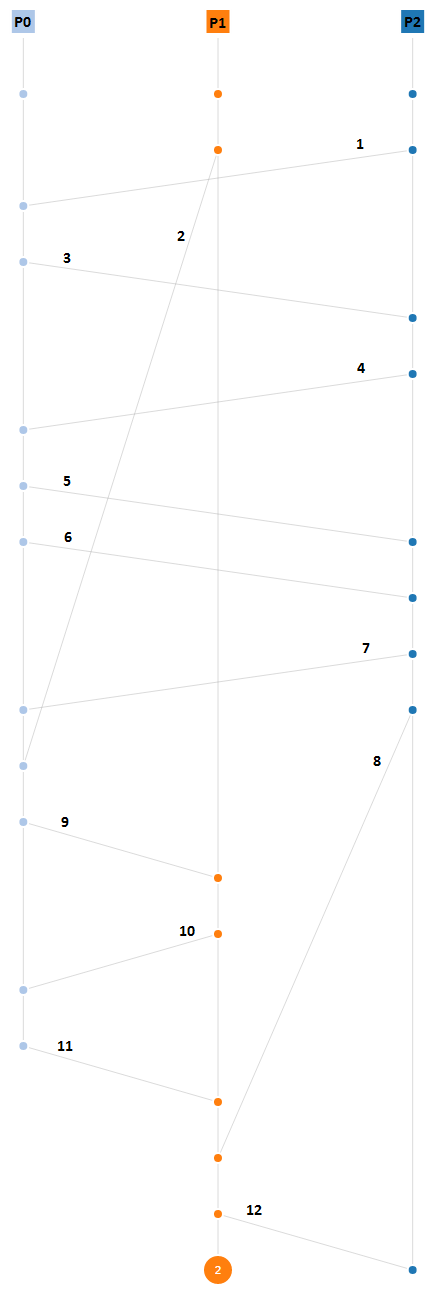
\includegraphics[width=0.4\textwidth]{report/images/shiviz_chord2}
  \caption{Shiviz log of a three peer Chord ring being constructed. \label{fig:shiviz_chord}}
\end{figure}

In the second scenario (figure \ref{fig:shiviz_article}), a Chord ring consisting of two peers P0 and P1 is constructed. The client C1 then executes a pull operation via its server daemon P1. Peer P0 starts as the initial member of the Chord ring.
\begin{enumerate}
  \item P1 initiates joining the network by requesting its successors from P0.
  \item P0 replies with its IP address as the only successor.
  \item P1 requests to be P0's predecessor.
  \item P0 responds to P1.
  \item P0 stabilizes the ring by requesting P1 be its predecessor.
  \item P1 responds.
  \item The client initiates an RPC pull operation by calling the lookup function on its local daemon C1.
  \item P1 determines that it does not have the requested article and so forwards the request to P0.
  \item P0's RPC returns to P1 with article found.
  \item P1's RPC returns to C1 with article found and the address of the node hosting the article, P0.
  \item C1 requests the article from P0.
  \item Finally, P0 returns the article to C1.
\end{enumerate}

\begin{figure}[tbh!]
  \centering
  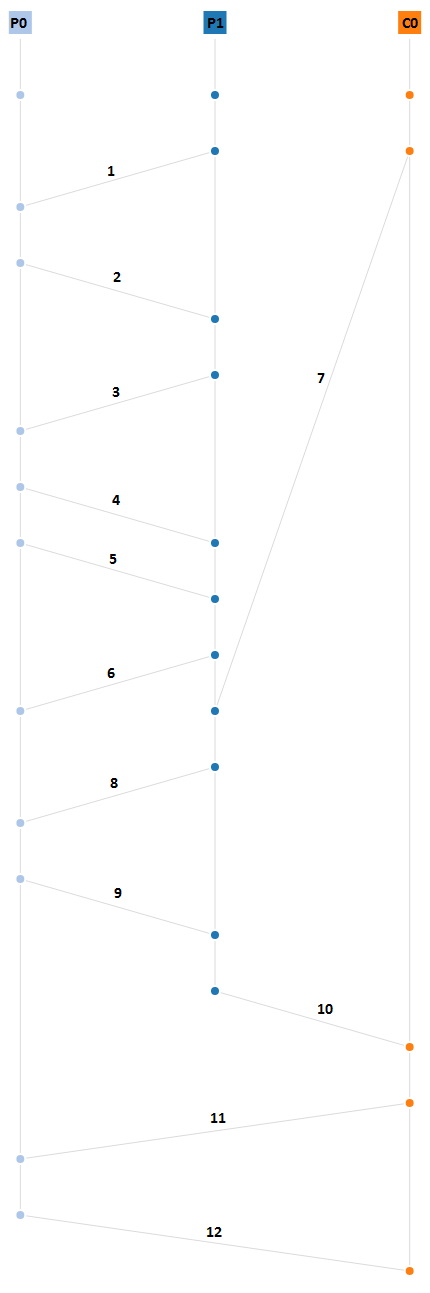
\includegraphics[width=0.4\textwidth]{report/images/shiviz_article1}
  \caption{Shiviz log of an article retrieval in a two peer Chord network. \label{fig:shiviz_article}}
\end{figure}


\section{Conclusion}
We have implemented a prototype peer-to-peer wiki using an enhanced version of Chord and the Treedoc CRDT. It is scalable and ensures articles are available and consistent while supporting disconnected editing at multiple sites. By using a CRDT, we were able to implement a caching mechanism to improve availability without incurring any additional communication costs and to implement replication of articles.

The client application provides a natural interface for interacting with articles. It exposes six opertations that allow users to retreive, view, modify, and update shared articles hosted on remote peers.

Further evaluation is needed to determine the number of peers supported on our system. The finger table optimization we implemented in our Chord library should ensure that the Chord network scales well. However, there are several other DHTs that have been proposed and may perform better than Chord in our use case. One example is Kademlia \cite{kademlia}, which uses a tree-based routing table. Another is P-Grid \cite{pgrid}, which is designed to support substring matches of the resource identifier which, in our case, is the article title.

\bibliographystyle{abbrv}
\bibliography{report}
\end{document}
